\documentclass[a4paper]{article}
\usepackage{natbib}
\usepackage{url}
\usepackage{hyperref}
\hypersetup{
    colorlinks,
    citecolor=black,
    filecolor=black,
    linkcolor=black,
    urlcolor=black,
	linktoc=all,
	bookmarksdepth=paragraph
}
\usepackage[cyr]{aeguill}
\usepackage[utf8]{inputenc}
\usepackage[francais]{babel}
\usepackage{amsmath}
\usepackage{graphicx}
\usepackage{parskip}
\usepackage{fancyhdr}
\usepackage{listings}

%%configuration de listings
\lstset{
	language=PHP,
	basicstyle=\ttfamily\footnotesize, %
	identifierstyle=\color{red}, %
	keywordstyle=\bfseries\color{blue}, %
	stringstyle=\color{black!60}, %
	commentstyle=\color{green!95!yellow!1}, %
	columns=flexible, %
	tabsize=2, %
	extendedchars=true, %
	showspaces=false, %
	showstringspaces=false, %
	numbers=left, %
	numberstyle=\tiny, %
	breaklines=true, %
	breakautoindent=true, %
	captionpos=b
}

\title{Réalisation d'un site de partage et de création de dessins}
\author{Lucien Aubert $\newline$ Tom Henoch}

\makeatletter
\let\theauthor\@author
\let\thetitle\@title
\makeatother

\pagestyle{fancy}
\fancyhf{}
\chead{\thetitle}
\cfoot{\raggedleft\thepage}
\begin{document}

\begin{titlepage}
	\centering
    \vspace*{0.5 cm}
    \href{http://iut.univ-amu.fr/sites/arles}{
\includegraphics[scale = 0.15]{logo-amu.png}}\\[1.0 cm]
    \textsc{\LARGE Aix-Marseille Université}\\[2.0 cm]
	\textsc{\Large M3103 - Programmation Web côté serveur}\\[0.5 cm]
	\rule{\linewidth}{0.2 mm} \\[0.4 cm]
	{ \huge \bfseries \thetitle}\\
	\rule{\linewidth}{0.2 mm} \\[1.5 cm]

	\begin{minipage}[t]{0.4\textwidth}
		\begin{flushleft} \large
			\emph{Auteurs :}\\
			\theauthor
			\end{flushleft}
			\end{minipage}~
			\begin{minipage}[t]{0.4\textwidth}
			\begin{flushright} \large
			\begin{flushleft}
			\emph{Enseignants :} \\
			Brett Desbenoit $\newline$Laurent Carmignac
		 \end{flushleft}
		\end{flushright}
	\end{minipage}\\[2 cm]

	\vfill
\end{titlepage}
\pagestyle{empty}
\tableofcontents
\pagebreak
\pagestyle{fancy}
\setcounter{page}{1}
\section{Introduction}
L'utilisateur sera en mesure de dessiner avec des outils basiques (crayon, carré, cercle, lettrages) et de partager sa création. Les dessins ainsi créés sont modifiables par plusieurs utilisateurs.

Les utilisateurs pourront commenter les dessins et les marquer comme "J'aime".

\section{Structure}
L'application est composée de trois modules qui interagissent :
\begin{itemize}
	\item un serveur web (site + base de données)
	\item un serveur spécifique à l'édition de dessin
	\item une application client servie par le serveur web
\end{itemize}

\begin{center}
	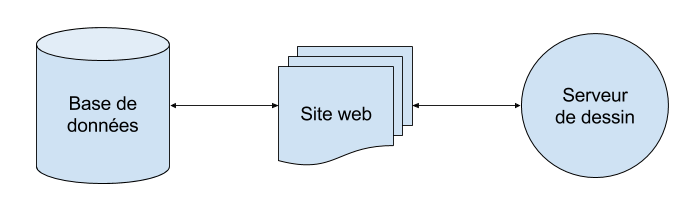
\includegraphics[width=0.8\textwidth]{sketcher_global_structure.png}
\end{center}

La base de données n'est accessible que par le site web, doté d'une API type REST permettant au serveur de dessin de lui passer des requêtes.

\subsection{Serveur Web}
Le site web est développé avec le framework \cite{Symfony}Symfony 3 et utilise une base de données MariaDB. Il est hébergé sur un serveur Apache 2.4.

Le moteur de template utilisé est Twig et l'ORM utilisé est Doctrine2.

Ce serveur joue les rôles d'interface utilisateur et d'interface entre le serveur de dessin et la base de données.

C'est lui qui donne la permission au serveur de dessin de démarrer une connexion avec un client.

\subsubsection{Connexion à la base de données}
Les paramètres de connexion à la base de données se trouvent dans le fichier \texttt{app/config/parameters.yml}.

Afin d'exécuter des requêtes SQL sur le serveur de base de donnée MariaDB nous utilisons la bibliothèque Doctrine fournie avec notre framework.

\subsubsection{Fonctions}
Pour l'utilisateur, le site permet de
\begin{itemize}
	\item s'inscrire
	\item se connecter (authentification par nom et mot de passe)
	\item créer un nouveau dessin
	\item consulter la galerie
	\item rechercher un dessin par nom
	\item rechercher un dessin par tag
	\item modifier son profil
	\item modifier ses dessins (titre, auteurs, tags)
\end{itemize}

\subsubsection{Plan du site}
\begin{center}
	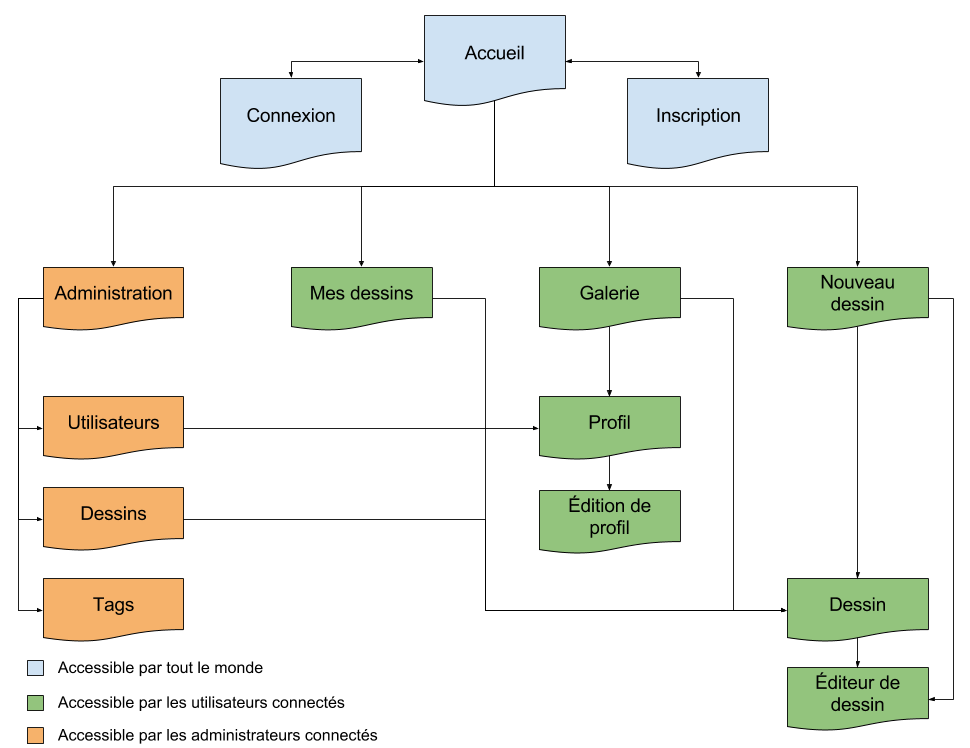
\includegraphics[width=1\textwidth]{sketcher_sitemap.png}
\end{center}

\vspace{10 mm}
Les pages protégées redirigent vers la page de connexion si l'utilisateur n'est pas connecté et vers la page d'accueil quand il tente d'accéder à du contenu qui ne lui est pas accessible.

\paragraph{Remarque}

Symfony aidant, il nous est possible de vérifier si l'utilisateur nous a donné le cookie d'une session grâce à cette simple condition, \texttt{\$this} étant notre controleur.
\begin{lstlisting}
if(!$this->getUser())
	return $this->redirectToRoute('login');
\end{lstlisting}

\subsubsection{Espace d'administration}
Le premier utilisateur (avec l'id 1), ou super-administrateur, et tous les administrateurs qu'il nommera peuvent accéder à un espace d'administration à partir duquel il peuvent supprimer et modifier les autres utilisateurs (et les autres administrateurs dans le cas du super-administrateur), les dessins et les tags.

L'accès à cet espace est restreint grâce au membre booléen \texttt{is\_admin} du modèle \texttt{User}. Si il est $vrai$ la requête est acceptée, sinon le client est redirigé vers la page d'accueil.

\begin{lstlisting}
if(!$user->getIsAdmin())
	return $this->redirectToRoute('homepage');
\end{lstlisting}

\subsubsection{Améliorations}
\paragraph{Intégration d'un éditeur Javascript: }L'application de dessin a été développée et intégrée au site. Voir le chapitre concerné plus bas.
\paragraph{Catégories avancées: }Pour chaque dessin les auteurs peuvent ajouter/supprimer des \textit{tags}. Il est possible d'afficher les dessins affiliés à un tag en cliquant sur l'un d'entre eux.
\paragraph{Notation: }Un système de \textit{J'aime} a été implanté. Chaque utilisateur peut aimer ou non un dessin. Les dessins sont classés par nombre de \textit{J'aime} dans la galerie.
\paragraph{Internationalisation: }Le site est traduit grâce au système de localisation Symfony.
\paragraph{Statut des utilisateurs: }Tous les noms d'utilisateurs écrits sur les pages du site sont accompagnées d'un macaron de couleur indiquant si l'utilisateur est connecté (vert) ou non (gris).


\subsubsection{Routage}
La chaîne \texttt{'login'} correspond ici à la route vers laquelle rediriger le client. Le système de routing du framework permet de définir des routes en leur attribuant un nom, des arguments et une méthode qui sera exécutée quand la route sera demandée par un client. Ces définitions sont faites sous forme de commentaires formatés comme suit.
\begin{lstlisting}
	/**
	* @Route(
	*   "/sketch/{sketchId}",
	*   requirements={"sketchId": "\d+"},
	*   name="sketch"
	* )
	*/
\end{lstlisting}
Les fichiers source sont ensuite traités par Symfony et les commentaires parsés pour produire un module de routage sur mesure.

\subsubsection{Feuilles de style et UX}
Afin de garantir un résultat similaire sur un maximum de navigateurs nous avons choisi d'utiliser un bootstrap appelé Kickstart. Cet outil nous apporte un CSS basique et un module Javascript permettant notamment l'affichage de notifications colorées dans le coin supérieur droit de l'écran.

\subsubsection{Ajax}
Nous avons privilégié des interfaces avancées pour certains formulaires (champs d'édition de tags, d'auteurs, de titre). Pour se faire nous avons eu recours à l'utilisation de \texttt{XMLHttpRequest}, une object Javascript qui permet de faire envoyer des requêtes HTTP par le client. Le client envoie donc des requêtes \texttt{GET} vers le serveur pour signaler l'ajout ou la suppression d'un tag ou d'un auteur, le serveur envoie sa réponse sous forme d'un fichier JSON avec une message d'erreur ou de succès qui sera parsé par le client pour afficher une notification.

Deux modules ont été développés pour permettre la validation des ces champs via des requêtes Ajax. Il s'agit des fichiers \texttt{web/js/tagInput.js} et \texttt{web/js/fastInput.js} qui sont initialisés dans les vues qui les utilisents (\texttt{app/Resources/views/show_sketch.html.twig} par exemple).

\subsection{Serveur de dessin}
Cet élément est développé en Javascript et est supposé être lancé avec le moteur \cite{NodeJS}NodeJS. Ce serveur fait la liaison entre l'application client de dessin et le serveur web. Elle s'occupe de transmettre les modifications aux utilisateurs qui modifient un même dessin.

L'utilisation du module Javascript Socket.io nous a permis de faire la liaison entre le client et le serveur de dessin.

\subsubsection{Authentification}
La consultation et la modification de la base de données par l'application client est permise par l'authentification de ce dernier auprès du serveur de dessin.

Le client se connecte au site web pour accéder à la page d'édition de dessin. La page lui est envoyée avec un jeton propre à cet utilisateur et à ce dessin. Le client lance l'application Javascript qui envoie le jeton au serveur de dessin. Le serveur de dessin s'occupe de vérifier le jeton en demandant sa validation au serveur web. Si le jeton est bon le client peut modifier le dessin et récupérer les changements faits dessus par les autres clients.

L'API que sert le serveur web n'acceptera aucune requête si le jeton envoyé avec est invalide. Ainsi, chaque commande passée par l'application client est authentifiée et, pourtant, passe par le serveur de dessin, qui peut donc assumer son rôle de diffuseur (\textit{broadcast}).

\subsubsection{Communication}
Pour communiquer tant avec le serveur web qu'avec le client nous utilisons le format JSON, dont l'utilisation est possible nativement en Javascript. Les retours du serveur web, les requêtes en provenance de l'application client ainsi que les retours et requêtes du serveur de dessins sont passées dans ce format, par le protocole HTTP.

\subsubsection{Upload de fichiers malveillants}
L'upload de fichier étant un point sensible d'une application web nous avons décidé d'endiguer le risque de présence de fichier malveillants sur le serveur en implantant dans le serveur de dessin les mêmes classes que dans l'application client afin de redessiner sur le serveur l'image produite par les utilisateurs. Ainsi aucun fichier de l'utilisateur ne peut être téléchargé sur le serveur.

\subsection{Application client}
L'application client consiste en une page HTML dans laquelle sont chargés différents modules Javascript regroupés dans \texttt{web/js/Sketcher} grâce au fichier \texttt{web/js/Sketcher/Sketcher.js}.

Elle se charge de permettre l'édition d'un dessin à partir des données (jeton de connexion, dimensions et données du dessin) présente dans la page. Elle communique directement avec le serveur de dessin à l'aide du module Javascript Socket.io après lui avoir envoyé le jeton de connexion.

\subsubsection{Canvas}
L'application client est basée sur la technologie \texttt{canvas} dont les navigateurs récent implémentent l'API de dessin. Nous dessinons dans un nœud DOM \texttt{<canvas>} à l'aide de méthodes telles que
\begin{lstlisting}
ctx.fillRect(0, 0, 20, 20);
ctx.strokeRect(0, 0, 20, 20);
\end{lstlisting}

\subsubsection{Sélection des couleurs}
Nous avons jugé préférable d'utiliser un module externe, \cite{ColorPicker}ColorPicker de Peter Dematté, pour permettre la sélection des couleurs.

\subsubsection{Format de données}
Afin de transmettre les nouveaux objets du dessin et de recevoir ceux diffusés par le serveur de dessin, nous utilisons un objet JSON.
\begin{lstlisting}
{
	width: 200,		// Pixels
	height: 200,
	layers: [
		{
			name: "Background",
			objects: [
				{
					"type": "Circle",
					"data": {
						"options": {
							"thickness": 5,		// Pixels
							"fill": true,
							"stroke": true
							},
						"p1": { "x": 100, "y": 100 },
						"p2": { "x": 150, "y": 150 },
						"stroke_color": "rgba(0, 0, 0, 1)",
						"fill_color": "rgba(95, 195, 29, 1)"
					}
				}
			]
		}
	]
}
\end{lstlisting}
Voici par exemple l'objet transmis par le client au serveur de dessin lors de l'édition d'un dessin de 200 pixels de large sur 200 pixels de haut contenant un cercle vert bordé de noir.

\section{Difficultés rencontrées}
La prise en main d'un framework aussi fourni que Symfony a été fastidieuse bien que les documentations du framework, de Twig et de Doctrine soient abondantes.

Le développement d'application avec communication asynchrone comme c'est le cas du serveur de dessin et de l'application client était un exercice nouveau. Il nous a fallu trouver des solutions (bibliothèques, serveurs) nous permettant d'atteindre nos objectifs et en apprendre l'utilisation.

\section{Conclusion}
La création de cette application nous a permis de découvrir le framework Symfony 3 ainsi que la technologie \cite{WebSockets}WebSocket. L'utilisation du Javascript pour le développement de l'outil de dessin nous a appris beaucoup sur ce langage, tant côté serveur que côté client.

Le déploiement de l'application a été un défi que nous avons relevé en nous documentant sur le serveur web que nous utilisions, Apache 2.4, ce qui nous a permis d'approfondir les connaissances que nous avons acquis en cours de réseau.
\newpage
\bibliographystyle{unsrt}
\bibliography{biblio}

\end{document}
